\chapter{Validation}
\label{chaper-3}

%Validation du simulateur avec exo 4 TP 1, sous forme de tableau comparatif à double entrée.....\\
%Détail calcul à la main...\\
%Tracé des rayons obtenus àpd simulateur...\\




Remarque: lors de la simulation de la situation de l'exercice 1 du TP4, nous ne pouvons pas utiliser la puissance sur une zone locale $<P_{RX}>$ (équation \ref{eq:puissance-locale}), mais bien $P_{RX}$ en un point de l'espace (équation \ref{eq:puissance-un-point}).
\begin{equation}
    \label{eq:puissance-un-point}
    P_{RX}\ = \frac{60 \lambda^2}{8 \pi^2 R_a}P_{TX}G_{TX} \left| \sum_{n=1}^N \Gamma_1 \Gamma_2 \Gamma_3 \dotsc T_1 T_2 T_3 \frac{e^{-j \beta d_n}}{d_n} \right|^2
\end{equation}

Le calcul du champ électrique utilise l'équation (\ref{eq:elec-field}).\\

L'exercice 1 du TP4 utilise un $P_{TX}G_{TX}=1,64$, une fréquence à $868,3 \mathrm{MHz}$, une résistance d'antenne $R_a=73 \Omega$, ainsi que des murs ayant comme permittivité relative $\varepsilon_r=4.8$ et comme conductivité $\sigma=0.018$.

\section{Calculs pour rayon à deux réflexions, cas A}
% Donnez le détail du calcul à la main l’une des composantes à deux réflexions, au choix (un exemple vous est donné pour une réflexion dans les corrigés)
...

\section{Comparaison calculs et simulation}
Nous pouvons comparer les résultats de notre simulateur avec les résultats calculés manuellement afin de valider notre implémentation. Un tableau comparatif [Table \ref{tab:comparaison-calculs-simulation}] présente ces données.

\begin{table}[H]
    \centering
    \begin{tabular}{|l|l|r|r|r|}
         \hline
                                  & Grandeur & Calculs & Simulation & Erreur \\
        \hline
\multirow{2}{*}{Direct}           & $\left|\underline{E}\right|$ [V/m] & $4,031\cdot10^{-3}$ & $4,0124\cdot10^{-3}$ & $0,40\%$ \\
                                  & $P_{RX}$ [W] & $3,33\cdot10^{-10}$  & $3,32965\cdot10^{-10}$ & $0,01\%$     \\
        \hline
\multirow{2}{*}{1 réflexion (A)}  & $\left|\underline{E}\right|$ [V/m] & $7,0819\cdot10^{-4}$ & $7,07611\cdot10^{-4}$ & $0,08\%$ \\
                                  & $P_{RX}$ [W] & $1,04\cdot10^{-11}$ & $1,03557\cdot10^{-11}$ & $0,42\%$ \\
        \hline
\multirow{2}{*}{1 réflexion (B)}  & $\left|\underline{E}\right|$ [V/m] & $6,7821\cdot10^{-4}$ & $6,78351\cdot10^{-4}$ & $0,02\%$ \\
                                  & $P_{RX}$ [W] & $9,53\cdot10^{-12}$ & $9,51694\cdot10^{-12}$ & $0,14\%$ \\
        \hline
\multirow{2}{*}{2 réflexions (A)} & $\left|\underline{E}\right|$ [V/m] & $4,4572\cdot10^{-4}$ & $4,46271\cdot10^{-4}$ & $0,12\%$ \\
                                  & $P_{RX}$ [W] & $4,11\cdot10^{-12}$ & $4,11896\cdot10^{-12}$ & $0,22\%$ \\
        \hline
%\multirow{2}{*}{2 réflexions (B)} & $\left|\underline{E}\right|$ [V/m] &   N/A   &      & N/A    \\
%                                  & $P_{RX}$ [W] &   N/A   &      & N/A    \\
%         \hline
    \end{tabular}
    \caption{Comparaison valeurs calculs et simulation selon le rayon}
    \label{tab:comparaison-calculs-simulation}
\end{table}

On peut observer que notre simulateur se rapproche beaucoup des valeurs réelles calculées à la main, avec une erreur ne dépassant pas 0,5\%. Ceci permet donc de valider l'implémentation de notre simulateur.

\section{Affichage simulation des rayons}

La Figure [\ref{fig:simu-tp4}] présente le tracé des rayons simulés. Le récepteur est représenté comme un carré bleu, l'émetteur comme un rond blanc, les points de réflexions comme des points magenta, les murs comme des traits gris, et les rayons sont différenciés par leur couleur représentant leur nombre de réflexions:
\begin{itemize}
    \item Vert: rayon direct (0 réflexion)
    \item Rouge: rayon à une réflexion
    \item Jaune: rayon à deux réflexions
\end{itemize}

\begin{figure}[H]
    \centering
    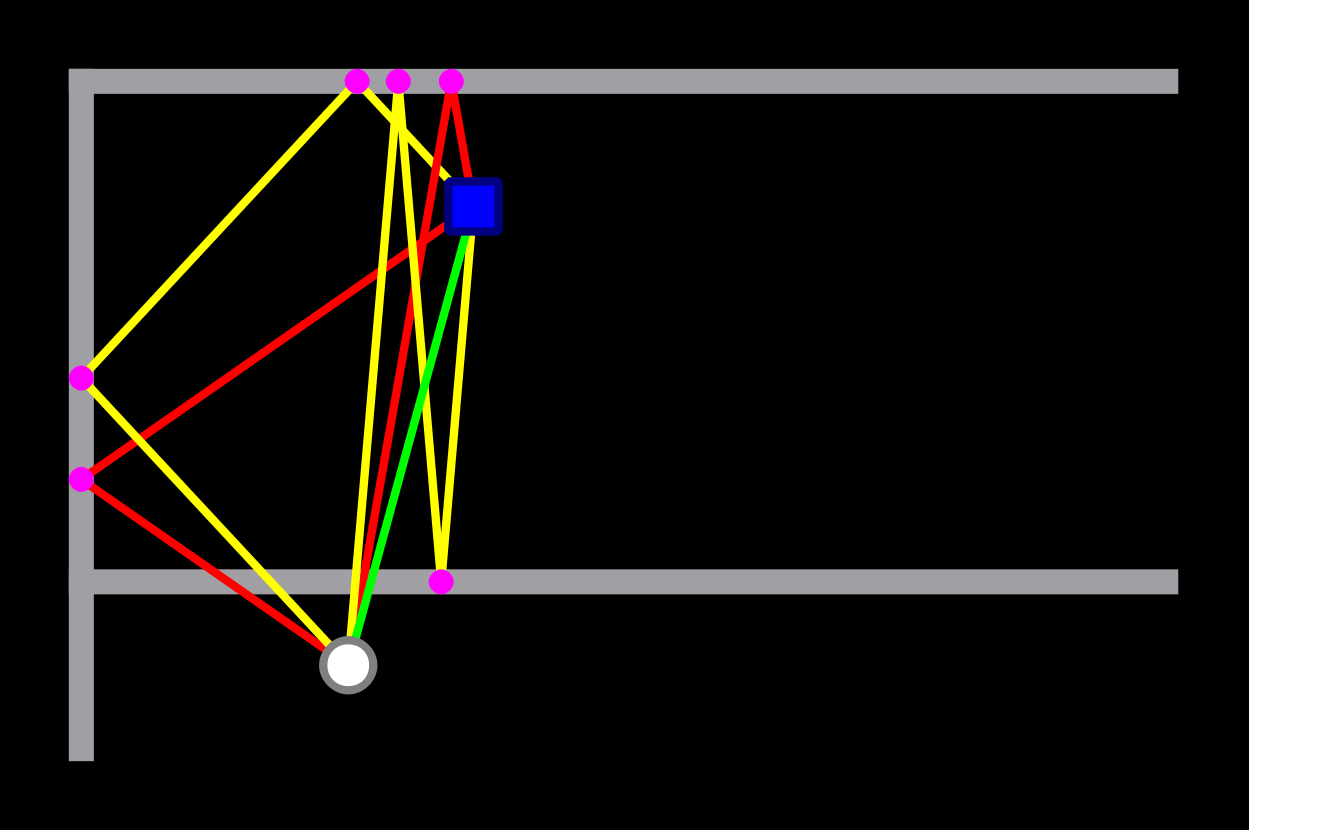
\includegraphics[width=\textwidth]{latex/images/tp4.png}
    \caption{Simulation Ray-Tracing de l'exercice 1, TP4}
    \label{fig:simu-tp4}
\end{figure}

Comme le simulateur complet de l'appartement, il est possible d'afficher plus d'informations du récepteur, tel que ses coordonnées ou encore sa puissance reçue, lors du survol de la souris par-dessus.
